\chapter{Umsetzung}

\section{Gesamt-Architektur}
Die Architektur besteht aus drei Hauptkomponenten: den Simulations-Engines, der Logging- und Visualisierungskomponente sowie dem BProgram, in dem Szenarien modelliert und ausgeführt werden können. Das BProgram kann zur Ausführung unabhängig zwischen den beiden bereitgestellten Simulations-Engines wählen. Innerhalb des Projekts wurden zunächst konkrete Szenarios manuell implementiert. Im weiteren Verlauf wurde ein Ansatz entwickelt, um konkrete Szenarien automatisiert zu erlernen, sodass diese einem abstrakt definierten Szenario folgen. In den konkreten Szenarien kommt zudem ein Logger zum Einsatz, der Daten für die Visualisierung bereitstellt. Diese Gesamtarchitektur ist in Abbildung \ref{fig:architecture} dargestellt.

\begin{figure}[h]
    \centering
    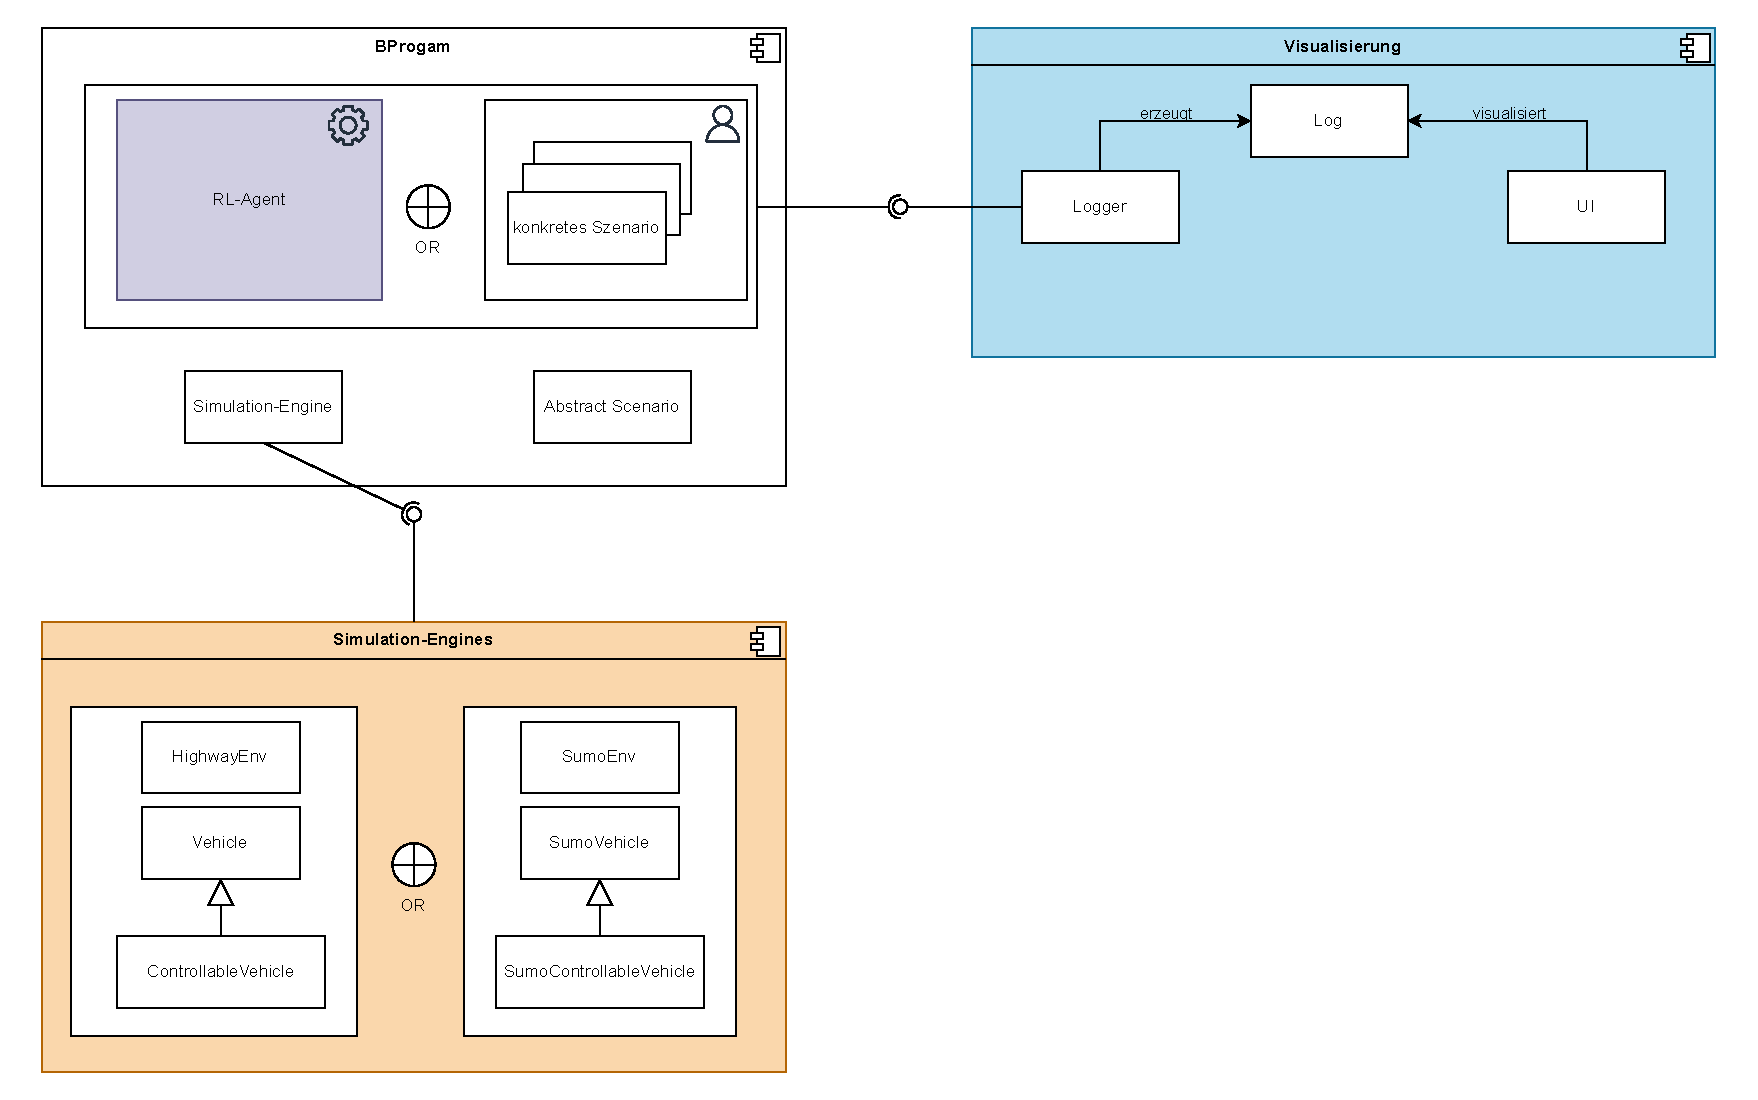
\includegraphics[width=0.95\linewidth]{contents/figures/fullArchitecture.pdf}
    \caption{Gesamtarchitektur}
    \label{fig:architecture}
\end{figure}

Im Folgenden werden zunächst die beiden Simulations-Engines sowie die Hilfsklassen vorgestellt, die den Zugriff auf Fahrzeuginformationen ermöglichen. Anschließend wird die Modellierung in BPpy erläutert, die verschiedene B-Threads für die Ausführung der Simulation, abstrakten Szenarien und konkreten Szenarien nutzt. Darauf folgt eine Beschreibung der Logging- und Visualisierungskomponente. Abschließend wird der Ansatz zum automatisierten Erlernen konkreter Szenarien auf Basis eines abstrakten Szenarios vorgestellt.

\section{Simulationsumgebungen}
In diesem Abschnitt wird die Nutzung von HighwayEnv und SUMO sowie dessen Steuerungsschnittstelle TraCI beschrieben. Zunächst wird die Konfiguration von HighwayEnv beschrieben sowie zwei Ansätze zur Extraktion von Fahrzeuginformationen aus der Umgebung. Danach wird auf die Sumo-Verwendung innerhalb des Projektes eingegangen.
\subsection{HighwayEnv}
\subsubsection{Konfiguration von HighwayEnv}
In unserem Projekt kommt die von HighwayEnv bereitgestellte Umgebung \texttt{highway-v0} zum Einsatz. Diese simuliert eine mehrspurige Fahrbahn und kann konzeptionell als Autobahnumgebung verstanden werden. 

Damit mehrere Fahrzeuge gleichzeitig steuerbar sind, muss die gewünschte Anzahl an kontrollierbaren Fahrzeugen über den Parameter \texttt{controlled\_vehicles} spezifiziert werden. Zusätzlich lassen sich weitere, nicht kontrollierte Fahrzeuge über den Parameter \texttt{vehicles\_count} in die Simulation integrieren. Ein spezielles VUT kann somit ebenfalls über diesen Mechanismus berücksichtigt werden.

Da unser Projekt in einem Multi-Agent-Setting ausgeführt wird, ist eine entsprechende Konfiguration notwendig. Hierfür müssen sowohl der Action-Typ (\texttt{MultiAgentAction}) asl auch der Observation-Typ (MultiAgentObservation) gesetzt werden. Auf diese Weise wird sichergestellt, dass:
\begin{enumerate}
    \item mehrere Agenten gleichzeitig Aktionen ausführen können und
    \item die Beobachtungsdaten (Observation) auch für alle kontrollierten Fahrzeuge bereitgestellt werden.
\end{enumerate}

\subsubsection{Ansätze zum Zugriff auf Fahrzeuginformationen}
\label{sec:get_vehicle_info}
Um in HighwayEnv Entscheidungen zu treffen, etwa hinsichtlich Abständen zwischen Fahrzeugen, Spurwahl oder Spurwechseln, ist eine geeignete Repräsentation von Fahrzeuginformationen erforderlich. In diesem Kapitel werden zwei unterschiedliche Ansätze vorgestellt. Zunächst der \texttt{ObservationWrapper}, anschließend ein Vehicle-basiertes Modell. Abschließend erfolgt ein Vergleich der beiden Methoden.

Der \texttt{ObservationWrapper} kapselt die von der Environment zurückgegebene Observation und interpretiert deren Werte fachlich. Zu Beginn einer Simulation wird dieser einmalig initialisiert und nach jedem Step mit den aktuellen Daten aktualisiert. Auf Basis dieser Struktur können Methoden, wie \texttt{is\_right\_lane\_} oder \texttt{get\_distance\_to\_leading\_vehicle} genutzt werden, um Abstände und Spurverfügbarkeit zu prüfen.

Ein zentrales Kriterium für Korrektheit ist dabei die Reihenfolge der Features innerhalb der Observation. In der aktuellen Implementierung müssen die Werte \verb|["x", "y", "vx", "vy"]| genau in dieser Abfolge am Anfang des Arrays stehen. Nur dann können Distanz- und Geschwindigkeitsberechnungen valide durchgeführt werden. Darüber hinaus ist der Zugriff auf das Environment selbst notwendig, da bestimmte Informationen, etwa die Struktur des Straßennetzes, nicht allein aus der Observation extrahiert werden können. So lassen sich etwa Lanes über die Road-Network-Struktur bestimmen, was zusätzliche Abfragen an die Environment erfordert. 

Damit wird eine relativ direkte Möglichkeit geboten mit den von HighwayEnv bereitgestellten Daten zu arbeiten. Gleichzeitig macht ihn die starke Abhängigkeit von der Feature-Reihenfolge und der Environment-Konfiguration anfälliger für Fehler.
\newline
\newline
Der zweite Ansatz modelliert Fahrzeuge explizit als Objekte. Dazu stehen die Klassen \texttt{Vehicle} und \texttt{ControllableVehicle} zur Verfügung.
\begin{enumerate}
    \item \texttt{Vehicle} repräsentiert ein nicht kontrolliertes Fahrzeug und kapselt Methoden, die Informationen direkt aus der Simulation extrahieren. Dazu gehören unter anderem \texttt{speed()}, \texttt{lane\_index()} sowie Distanzwerte wie \texttt{delta\_pos} oder \texttt{delta\_x\_pos()}. Zusätzlich lassen sich Relationen wie \texttt{is\_ahead\_of()} oder \texttt{is\_behind()} zwischen zwei Fahrzeugen prüfen.
    \item \texttt{ControllableVehicle} erweitert die Funktionalität um konkrete Aktionsmöglichkeiten. Ein solches Fahrzeug kann über Aktionen wie LANE\_LEFT, LANE\_RIGHT, FASTER, SLOWER oder IDLE direkt gesteuert werden. Damit bildet es die Schnittstelle zwischen Entscheidungslogik und HighwayEnv.
\end{enumerate}

Die Objekte werden beim Start der Simulation einmalig erzeugt und behalten anschließend den Zugriff auf die von ihnen zugeordneten Fahrzeuge. Eine explizite Aktualisierung interner Variablen ist nicht erforderlich, da die Methoden unmittelbar auf die jeweils aktuellen Daten der Environment zugreifen.

Im direkten Vergleich erweist sich der Vehicle-basierte Ansatz als robuster und flexibler, da die Objekte nur einmalig instanziiert werden und ihre Methoden jederzeit aktuelle Daten liefern, entfällt die Gefahr inkonsistenter Zustände. Der \texttt{ObservationWrapper} hingegen ist stärker fehleranfälligm denn er ist auf die exakte Reihenfolge der Features in der Observation angewiesen und bei Änderungen der Konfiguration können ungültige Ergebnisse geliefert werden.

\subsection{Sumo}
Im Verlauf des Projektes zeigte sich, dass die Definition eines eigenen Straßennetzes in HighwayEnv über die Implpementierung einer individuellen Environment erfolgen muss. Daher wurden alternative Lösungen untersucht, was uns zur Verkerhssimulation SUMO führte. In SUMO können individuelle Karten einfach mit SUMO-netedit erstellt werden. Zudem bietet die Software die Möglichkeit, Straßennetze auf Basis realer Straßen zu generieren.
\subsubsection{SumoEnv}
Im Gegensatz zu HigwhayEnv bietet SUMO keine direkte Implementierung einer \texttt{gym.Env}-Umgebung. Um dennoch Reinfocement-Learning-Experimente in SUMO durchführen zu können wurde eine eigene Umgebung in der Klasse \texttt{SumoEnv} entwickelt. Diese basiert auf dem Gymnasium-Framework und bildet die standardisierten Methoden \texttt{reset}, \texttt{step}, \texttt{close} sowie die Definition von Beobachtungs und Aktionsräumen ab. Voraussetzung für die Nutzung ist die Installation von SUMO sowie das Python-Package TraCI, das eine bidirektionale Steuerung der SUMO-Simulation erlaubt.

Der Konstruktor übernimmt die Initialisierung der Umgebung. Neben der Referenz auf die SUMO-Konfigurationsdatei werden steuerbare Fahrzeuge als Parameter übergeben. Zudem werden die für das Reinforcement Learning relevanten Schnittstellen definiert:
\begin{itemize}
    \item \textbf{Beobachtungsraum}: Als \texttt{spaces.Box} modelliert, repräsentiert er kontinuierliche Werte und ist in der aktuellen Version als Matrix der Dimension (20, 5) umgesetzt.
    \item \textbf{Aktionsraum}: Über \texttt{spaces.MultiDiscrete} werden diskrete Handlungsoptionen für jedes steuerbare Fahrzeug definiert. Dies ermöglicht eine flexible Steuerung mehrerer Agenten gleichzeitig.
\end{itemize}
Zur Verwaltung des Simulationsverlaufs werden Episoden- und Schrittzähler geführt (\texttt{episode}, \texttt{step\_count}, \texttt{max\_steps}).

Zum Starten der Simulation wird in \texttt{start\_simulation} zunächst geprüft, ob die Umgenungsvariable \texttt{SUMO\_HOME} gesetzt ist, um die ausführbare SUMO-Datei korrekt zu lokalisieren. Die Verbindung zu SUMO wird anschließend über TraCI hergestellt. Danach werden Parameter zur Zeitschrittlänge, Kollisionsbehandlung und Startoptionen gesetzt. In der GUI werden zudem Kameraeinstellungen angepasst, um die Simulation bestmöglich visuell nachvollziehen zu können.

Das Hinzufügen von Fahrzeugen übernimmt \texttt{build\_vehicle}. Neben einem vordefinierten Vehicle under Test (vut) werden alle übergebenen steuerbaren Fahrzeuge erzeugt. Mit den individuellen Eigenschaften wie Startzeit, Fahrspur, Geschwindigkeit, Route oder Fahrverhalten können diese weiter angepasst werden. Besonders hervorzuheben ist, dass der Spurwechsel- und Geschwindigkeitsmodus der kontrollierbaren Fahrzeuge so gesetzt wurde, dass möglichst wenige Sicherheitsfeartures von SUMO aktiv sind. Auf diese Weise greifen SUMO-interne Automatikmechanismen, die Fahrmanöver einschränken oder korrigieren, nur minimal ein. 

Ein Neustart der Umgebung erfolgt über \texttt{reset}. Falls bereits eine Simulation aktiv ist, wird diese zunächst beendet (\texttt{close}). Danach erfolgt ein Neustart der SUMO-Instanz sowie die Einbindung der Fahrzeuge. Eine kurze Verzögerung sorgt dafür, dass die Setup-Phase abgeschlossen ist, bevor auf die Fahrzeuge zugegriffen wird, um Fehler bei der Ausführung zu vermeiden.

Innerhalb der \texttt{step}-Methode wird der eigentliche Iterationszyklus einer Episode ausgeführt. Dieser besteht aus:
\begin{enumerate}
    \item Anwendung der Agentenaktionen
    \item Fortsetzung der Simulation um einen Zeitschritt
    \item Erhebung der Beobachtung
    \item Berechnung der Belohnung
    \item Prüfung des Episodenendes
\end{enumerate}
Das Rückgabeformat entspricht dem Gymnasium-Standard: (obs, reward, terminated, truncated, info).

Die Aktionslogik (\texttt{\_apply\_action}) implementiert die fünf aus HighwayEnv bekannten diskreten Handlungsoptionen: LANE\_RIGHT, IDLE, LANE\_LEFT, FASTER und SLOWER. Die Beobachtungslogik sammelt hierbei für jedes Fahrzeug relevante Zustandsgrößen wie Geschwindigkeit und Position. Fehlerfälle (etwa aus der Simulation entfernte Fahrzeuge) werden abgefangen, indem Default-Werte zurückgegeben werden.

Die Belohnungsfunktion ist aktuell als Platzhalter implementiert und gibt einen konstanten Wert zurück. Damit ist die Umgebung lauffähig, ohne dass bereits eine spezifische Optimierungslogik definiert werden muss. In unserem Anwendungsfall liegt der Fokus ohne hin nicht auf der Optimierung der Simulation, sondern auf der Steuerung der Fahrzeug, die später einem abstrakten Szenario folgen sollen. Weitere Platzhalter-Methoden wie \texttt{\_get\_info}, \texttt{render} oder \texttt{\_render\_frame} sind vorgesehen, um die Funktionalität um detaillierte Diagnoseinformationen oder zusätzliche Visualisierungen zu erweitern. Innerhalb unserer Experimente war dies bisher nicht notwendig.

Die Methode (\texttt{close}) beendet die TraCI-Verbindung und sorgt für einen sauberen Abschluss der Simulation. Dies ist insbesondere für die korrekte Durchführung mehrerer Episoden im Training notwendig.
\subsubsection{Abbildung der Fahrzeugeigenschaften}
Wie bereits in Abschnitt \ref{sec:get_vehicle_info} gezeigt, hat sich der Vehicle-basierte Ansatz als robust und flexibel herausgestellt. Daher wurde er auch im Kontext von SUMO übernommen.

Zu diesem Zweck wurden die Klassen \texttt{SumoVehicle} und \texttt{SumoControllableVehicle} implementiert. \texttt{SumoVehicle} repräsentiert dabei nicht kontrollierte Fahrzeuge und stellt Methoden zur Verfügung, um relevante Fahrzeuginformationen direkt aus der SUMO-Simulation zu extrahieren. \texttt{SumoControllableVehicle} erweitert diese Funktionalität um konkrete Aktionsmöglichkeiten, die analog zur \texttt{ControllableVehicle}-Klasse im Kontext von HighwayEnv implementiert sind.

Durch diese Struktur müssen bestehende Szenario-Implementierungen lediglich einmalig auf die neue Simulations-Engine und die entsprechenden Fahrzeugobjekte angepasst werden. Die eigentliche Steuerungslogik kann unverändert übernommen werden. Gleichzeitig ermöglicht dieser Ansatz einen schnellen Wechsel der Simulations-Engine, sodass das Experiment-Setup nicht an eine spezifische Plattform gebunden ist udn flexibel zwischen HighwayEnv und SUMO oder anderen kompatiblen Umgebungen adaptiert werden kann.

\section{Modellierung von Szenarien mit BPpy}
Für die Modellierung von Szenarien wurde BPpy genutzt. Hierbei wurden verschiedene BThreads erstellt, die unterschiedliche Aspekte der Szenarien abbilden.
Einzelne BThreads bilden bestimmte Funktionalitäten und Teilszenarien ab, die dann in Kombination ein vollständiges, konkretes Szenario ergeben. So können die Funktionalitäten insgesamt besser strukturiert und wiederverwendet werden.
Die BThreads werden aber außer für einzelne Funktionalitäten auch für die Simulation und Abstraktion von Szenarien genutzt, sowie gebündelt um ein konrektes Szenario wie ein Überholmanöver abzubilden.
So gibt es BThreads, die ein abstraktes Szenario modellieren, also die grundlegende Anforderungen an das Szenario definieren, ohne sich auf eine konkrete Implementierung festzulegen. Diese abstrakten Szenarien werden dann im BProgram mit ausgeführt um zu überprüfen, dass die Anforderungen an das Szenario erfüllt werden.
Dabei werden konkrete Angaben überprüft, wie z.B. das sich bestimmte Fahrzeugpositionen verändert haben, oder in welcher Fahrbahn sich die Fahrzeuge im Vergleich zueinander befinden.
Dazu kann dann geloggt werden, ob die Anforderungen erfüllt wurden, und wenn nicht, welche Anforderungen nicht erfüllt wurden.

Der Simulations-Thread hat die Aufgabe, die Simulation zu steuern und sicherzustellen, dass die Szenarien in der Simulationsumgebung korrekt ausgeführt werden. Er sorgt dafür, dass die Fahrzeuge entsprechend den definierten Szenarien agieren und interagieren.
Dabei erhält der Simulations-Thread Informationen von den anderen BThreads, um die Simulation entsprechend anzupassen und zu steuern. Z.B. werden in diesem Thread Aktionen der Fahrzeuge ausgeführt, die von anderen BThreads definiert wurden.
Dieser Thread dient insbesondere der korrekten Übersetzung der Aktionen für die jeweilige Simulationsumgebung, die in diesem Integrationsprojekt entweder HighwayEnv oder Sumo sein kann.
In diesem Thread wird auch auf Kollisionen und andere terminierende Ereignisse geprüft, um die Simulation entsprechend zu beenden oder anzupassen.

Das konkrete Szenario wird durch die Kobination von verschiedenen BThreads modelliert, die zusammen die vollständige Logik und Anforderungen des Szenarios abbilden. Dabei wird spezifische Logik implementiert, die nur für dieses Szenario relevant ist und meist in weitere Methoden ausgelagert wird.
Die entsprechende Logik wird dann im relevanten BThread aufgerufen, um einen Teil des Szenarios zu steuern. Dabei können mehrere BThreads auch zu einem konkreten Szenario gehören, um verschiedene Aspekte abzudecken.
Diese Threads können über ein Paralleitätskonstrukt parallel ausgeführt werden, um die gleichzeitige Ausführung verschiedener Aspekte des Szenarios zu ermöglichen. Spezifische Logik wird in den einzelnen BThreads per \texttt{yield from} aufgerufen, um diese anzuwenden.

Die Aufteilung und Aufgaben der einzelnen BThreads wird jetzt noch einmal an einem konkreten Beispiel, dem Follow-Behind-Szenario, erläutert.
\subsection{Follow-Behind-Szenario}
Das Follow-Behind-Szenario modelliert eine Situation, in der ein oder mehrere Fahrzeuge einem anderen Fahrzeug (VUT) folgt. Dabei wird überprüft, ob das folgende Fahrzeug einen sicheren Abstand zum vorausfahrenden Fahrzeug einhält.
Dabei wird auch geprüft, ob dieses Szenario in einer bestimmten Zeit abgeschlossen wird, sodass alle Nicht-VUT-Fahrzeuge sich hinter dem VUT und in derselben Fahrbahn befinden.
Diese Anforderungen stellen die grundlegenden Anforderungen an das Szenario dar, die in einem abstrakten BThread modelliert werden. Das enstsprechende abstrakte Szenario wird mit geringen Anforderungen (nur die Positionierung in einer vorgegebenen Zeit) in der Methode \texttt{abstract\_scenario\_two\_vehicles\_follow\_vut} modelliert.
Das abstrakte Szenario mit den zusätzlichen Anforderungen an die Fahrbahnpositionierung wird in der Methode \texttt{abstract\_scenario\_2} modelliert.
\begin{lstlisting}[language=Python, caption=bstraktes Szenario: Zwei Fahrzeuge folgen dem VUT]
@thread
def abstract_scenario_two_vehicles_follow_vut():
    def condition():
        return v1.is_behind_by_x(vut) and v2.is_behind_by_x(v1)  # TODO: Same lane?

    satisfied = yield from await_condition(condition, 10)
    if satisfied:
        print("################ SAT")
    else:
        print("################ UNSAT")
\end{lstlisting}

Der Simulations-Thread sorgt dafür, dass die Fahrzeuge entsprechend den definierten Szenarien agieren und interagieren. Dabei erhält der Simulations-Thread Informationen von den anderen BThreads, um die Simulation entsprechend anzupassen und zu steuern.
In diesem Beispiel interagiert der Simulations-Thread mit Sumo um die Aktionen korrekt für die Umgebung zu übersetzen und auszuführen. In früheren Beispielen wurde dies auch für HighwayEnv umgesetzt.
Der Simulations-Thread prüft auch auf Kollisionen und andere terminierende Ereignisse, um die Simulation entsprechend zu beenden oder anzupassen. Zudem wird für alle Fahrzeuge der Simulation geprüft, ob gültige Aktionen vorliegen, die dann las Tupel an \texttt{step}-Methode übergeben werden.
Die Simulation wird über die step-Methode der Umgebung ausgeführt, die die Aktionen der Fahrzeuge verarbeitet und den Zustand der Simulation aktualisiert. Zuletzt wird die Anzahl an Schritten der Simulation erhöht.
\begin{lstlisting}[language=Python, caption=Simulations-Thread Beispiel SumoEnv]
@thread
def sumo_env_bthread():
    global step_count
    while True:
        # set vehicle_id to one of in this scenario to let it the gui follow that vehicle
        # vut, veh_manual_1, veh_manual_2
        traci.gui.trackVehicle("View #0", "veh_manual_1")
        collisions = traci.simulation.getCollisions()
        if collisions:
            print("Collision detected! Exiting simulation...")
            traci.close()
            raise SystemExit()

        e = yield sync(waitFor=true)

        actions = []
        for vehicle in controllable_vehicles:
            action_vehicle = e.eval(vehicle.vehicle_smt_var)
            if action_vehicle in action_map:
                actions.append(action_map[action_vehicle])
            else:
                actions.append(4)  # default is IDLE
        actions_tuple = tuple(actions)

        obs, reward, truncated, terminated, _ = env.step(actions_tuple)
        print(f"OBSERVATION in step {step_count}: {obs}")
        step_count += 1
\end{lstlisting}


\begin{lstlisting}[language=Python, caption=Simulations-Thread Beispiel HighwayEnv]
@thread
def highway_env_bthread():
    global step_count
    while True:
        evt = yield sync(waitFor=true)
        logger.debug(
            f"highway_env_bthread: step_count: {step_count}, action: {evt.eval(v1.vehicle_smt_var)}"
        )
        action_val = evt.eval(v1.vehicle_smt_var)
        if action_val == LANE_LEFT:
            action_index = 0
        elif action_val == LANE_RIGHT:
            action_index = 2
        elif action_val == FASTER:
            action_index = 3
        elif action_val == SLOWER:
            action_index = 4
        else:
            action_index = 1  # IDLE
        env.step(action_index)
        step_count += 1
        env.render()
\end{lstlisting}


Das konkrete Szenario ist in zwei BThreads gekapselt, die zusammen die vollständigen Anforderungen des Szenarios abbilden. Der erste Teil der Szenario-Logik in dient dazu, dass ein spezifisches Fahrzeug einem anderen Fahrzeug folgt. Die methode nimmt auch eine optionale Verzögerung in Sekunden an.
Die konkrete Logik, die für diesen Teil des Szenarios benötigt wird, wird über \texttt{yield from} aufgerufen, um die Logik für \texttt{follow\_behind} anzuwenden. In der Methode follow_behind wird zuerst die Methode \texttt{get\_behind} aufgerufen, die eine Wrapper-Methode für einzelne Logik-bausteine darstellt.
Daraus wird Logik aufgerufen, die dafür sorgt dass das Fahrzeug hinter ein amderes Fahrzeug zurückfällt und in die gleiche Fahrbahn wechselt. Dann wird die dadurch entstehende Distanz zwischen den Fahrzeugen minimiert, indem die Geschwindigkeit des folgenden Fahrzeugs distanzabhängig angepasst wird.
Zuletzt um das Szenario mit zwei folgenden Fahrzeugen hinter einem VUT abzuschließen, werden in der Methode \texttt{concrete\_scenario\_two\_vehicles\_follow\_vut} zwei BThreads parallel ausgeführt, die jeweils ein Fahrzeug hinter dem VUT folgen lassen.
Das Ergebnis ist dass sich zunächst ein Fahrzeug hinter dem VUT positioniert, und sobald dies erreicht ist, das zweite Fahrzeug sich hinter dem ersten Fahrzeug positioniert. Danach wird für die Fahrzeuge auch der Abstand und die angepasste Geschwindigkeit gehalten.
\begin{lstlisting}[language=Python, caption=Konkretes Szenario: Zwei Fahrzeuge folgen dem VUT - Relevante BThreads]
@thread
def follow_behind(
    behind_vehicle: SumoControllableVehicle,
    in_front_vehicle: SumoVehicle,
    delay_seconds: float = 0.0,
):
    # " serial: "
    # yield from wait_seconds(delay_seconds)
    yield from get_behind(behind_vehicle, in_front_vehicle)
    yield from stay_behind(behind_vehicle, in_front_vehicle)


@thread
def two_vehicles_follow_vut():
    yield from parallel(follow_behind(v1, vut), follow_behind(v2, v1))
\end{lstlisting}

\section{Visualisierung von ausgeführten konkreten Szeanrien}
\section{Reinforcement Learning}
Hier wird die Struktur und Funktionalität des Projekts, das ein Reinforcement-Learning-Modell (RL) für Überholszenarien trainiert, speichert und nutzt beschrieben. Die Hauptkomponenten des Projekts sind in mehreren Python-Dateien organisiert.

\texttt{src/envs/overtake\_env.py}
Diese Datei definiert die Umgebung für das Überholszenario, bei dem das VUT zum Überholen des vom Modell gesteuerten Fahrzeugs angeregt werden soll. Sie basiert auf einer Kernumgebung und erweitert diese um spezifische Logik für das Training eines RL-Agenten.
Analog existiert die Datei \texttt{src/envs/intersection\_env.py}, bei dem eine Umgebung für ein Kreuzungsszenario definiert wird.

\begin{itemize}
    \item \texttt{\_\_init\_\_(render\_mode, **config\_overrides)}: Initialisiert die Umgebung mit dem übergebenen Rendermodus. Zusätzlich kann die Konfiguration der Umgebung über den \texttt{config\_overrides} Parameter überschrieben werden.
    \item \texttt{reset(**kwargs)}: Setzt die Umgebung zurück, initialisiert die Position und Geschwindigkeit des Agenten sowie des zu überholenden Fahrzeugs (VUT).
    \item \texttt{step(action)}: Führt einen Schritt in der Umgebung aus, basierend auf der Aktion des Agenten. Berechnet Belohnungen anhand des Zustandes der Simulation, unter anderem der Position der Fahrzeuge im Vergleich zueinander. Abschließen wird überprüft, ob die Episode beendet ist. 
    \item \texttt{render()}: Rendert die Umgebung.
\end{itemize}

\texttt{src/main.py}
Diese Datei enthält den Einstiegspunkt für die Ausführung des Projekts und die Konfiguration der Umgebung.

\begin{itemize}
    \item \texttt{create\_env(config: Dict[str, Any])}: Erstellt eine neue Umgebung basierend auf der übergebenen Konfiguration.
    \item \texttt{set\_config()}: Definiert die Konfiguration der Umgebung, einschließlich Fahrspuren, Fahrzeugpositionen und Beobachtungs-/Aktionsräume.
    \item \texttt{main()}: Führt die Hauptlogik aus, einschließlich der Initialisierung der Umgebung und der Simulation von Aktionen.
\end{itemize}

\texttt{src/training/train\_overtake\_agent.py}
Diese Datei ist für das Training des RL-Modells verantwortlich.

\begin{itemize}
    \item \texttt{make\_env(rank: int)}: Erstellt eine Instanz der Überholumgebung für das Training.
    \item \texttt{RenderCallback}: Eine Callback-Klasse, der die Umgebung während des Trainings in regelmäßigen Abständen rendert. Ihre \texttt{\_on\_step()} Methode wird vom Modell während des Trainings aufgerufen um zu bestimmen ob die aktuelle Episode gerendert werden soll.
    \item \texttt{main()}: Führt das Training des RL-Modells durch. Es initialisiert das Modell und definiert die Traingsumgebung, trainiert es mit der \texttt{DQN}-Methode und speichert das trainierte Modell.
\end{itemize}

\subsection{Trainieren des Modells}
Das Training erfolgt in der Datei \texttt{train\_overtake\_agent.py}. Die Hauptschritte sind:
\begin{enumerate}
    \item Initialisierung der Umgebung mit \texttt{DummyVecEnv}, welchem das zu lernende Szenario übergeben wird.
    \item Definition des RL-Modells mit \texttt{DQN}. Dabei werden diverse Parameter wie der Diskontierungsfaktor für das Lernen des Modells festgelegt.
    \item Start des Trainings mit \texttt{model.learn()}.
\end{enumerate}

\subsection{Speichern des Modells}
Das trainierte Modell wird mit einem Zeitstempel versehen und im Verzeichnis \texttt{models/} gespeichert:
\begin{lstlisting}
model.save("models/overtake_dqn.zip" + current_time)
\end{lstlisting}

\subsection{Nutzen des Modells}
Das gespeicherte Modell kann später geladen und für Inferenz oder weitere Trainingsschritte verwendet werden:
\begin{lstlisting}
from stable_baselines3 import DQN
model = DQN.load("models/overtake_dqn.zip")
\end{lstlisting}